\section{开始撰写论文}
在\LaTeX 中论文的组织形式是严格按照结构化写作的方式展开的,章节之间层次分明,段落之间关系紧密。要做到这一点就需要熟悉结构化写作的一般过程,首先需要通过\TeX 命令定义各章节的标题。
\begin{verbatim}
\section{开始撰写论文}              %对应为  第2章 开始撰写论文
\subsection{标题与正文格式控制}     %对应为   2.1 标题与正文格式的控制 
\subsubsection{字体的控制命令}      %对应为   2.1.1 字体的控制命令
\end{verbatim}
由于采用了\verb|ctex|的\verb|article|类作为论文的基本类,所以定义标题的层级最多为二级标题。当你的论文出现三级标题如\verb|2.1.1.1|的时候,请考虑修改文章层级结构以适应格式化排版的要求。(四级标题多出现于书籍以及科技专著中,毕业论文作为文档类其出现此类三级标题的情况较为罕见)。在一个低级标题之后出现的一个高级标题会使得文档当前内容跳出作用域,通过这样的方式整个文章的整体脉络就可以很清晰地显现出来。
\subsection{字体字号的控制}
字体字号的处理是借助了\href{http://mirror.hust.edu.cn/CTAN/language/chinese/ctex/doc/ctex.pdf}{ctex}宏包实现的,仔细阅读该文档你能在中文格式处理方面节省许多时间。在宏包中对于处理字体和字号的方法进行详细的阐述。在我们熟知的排版系统中,形式和内容是一个密不可分的整体,两者相生相伴无法分离。从我们写下一段话,并选中这段话然后再设定字体和字号开始形式已经开始附加到我们想要表达的内容中了。但是在\LaTeX 中,所有的内容(也就是正文及相关附录)是不包含任何关于格式的信息的。这样就做到了形式与内容的彻底分离,是\LaTeX 区别于任何一个排版系统的根本原因。

实现内容与形式的剥离是一个痛苦的过程,我们需要摒弃我们懒惰的直觉并开始高度抽象化的思考,通过这样一个过程等到内容与形式再度统一。
\subsubsection{字体}
根据中文汉字支持宏包ctexart的参考文档,模板中预置的常用字体一共有五种,他们分别是:宋体,黑体,仿宋,楷书, 隶书。对应的控制方式如下:
\begin{center}
\begin{tabular}{ccccc}
\hline \rule[-2ex]{0pt}{5.5ex} { 宋体} & { 黑体} & { 仿宋} & { 隶书} & {楷书} \\ 
\hline \rule[-2ex]{0pt}{5.5ex} \textbackslash songti &\textbackslash  heiti  & \textbackslash fangsong & \textbackslash lishu & \textbackslash kaishu \\ 
\hline 
\end{tabular}  
\end{center}
这些字体基本满足了武汉理工大学本科生毕业论文中所要求的字体的需求。


\subsubsection{字号}
使用\verb|\zihao{4}|命令来规定四号字体,在前面加负号表示小四\verb|\zihao{-4}|.
\subsection{图片及表格的处理}

\subsubsection{在文档中加入图片}
理论上\LaTeX 可以处理各种各样的图片类型从jpeg到bmp,从pdf到eps都是可以接受的图片处理类型。选择合理的图片类型会提高论文的整体观感,使得最终的排版效果更为优良。而其中以无损压缩格式为优先推荐,原生pdf图片,原生eps图片都是最优的选择。如果实在无法找到矢量图,可以退而求其次地采用png图片或者jpeg格式的图片。
\begin{itemize}
\item \textbf{取人玫瑰手留余香}~~~~使用他人图片时记得标注出处和明显的引用。
\item \textbf{掌握一种数据绘图软件}~~~~Python, MATLAB, Mathematica 都是不错的选择
\item \textbf{探索示意图绘制的方法}~~~~指的是流程图,二维或三维线图,推荐Ipe editor, TiKZ, 以及 Microsoft Visio Ink-scape
\end{itemize}
图片插入范例
\begin{figure}[thbp!]
\centering
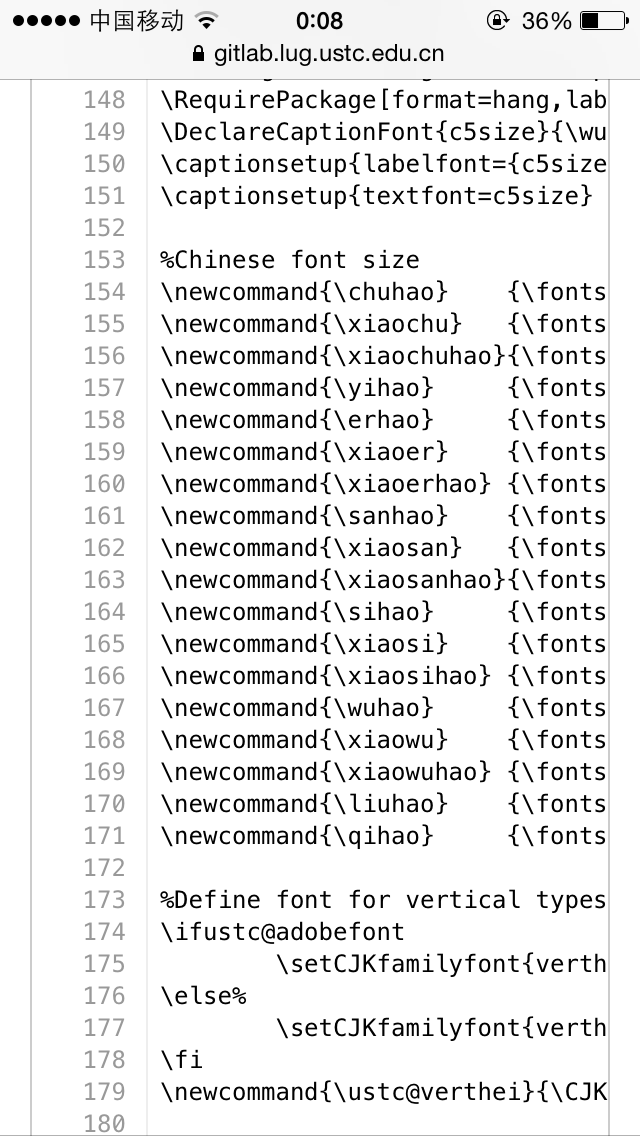
\includegraphics[width=0.4\linewidth]{figure/IMG_1832}
\caption{\LaTeX 字号错误使用范例}
\label{fig:IMG_1832}
\end{figure}

为了插入这样的图片,我们使用了如下的代码:
\begin{verbatim}
\begin{figure}[thbp!]
\centering
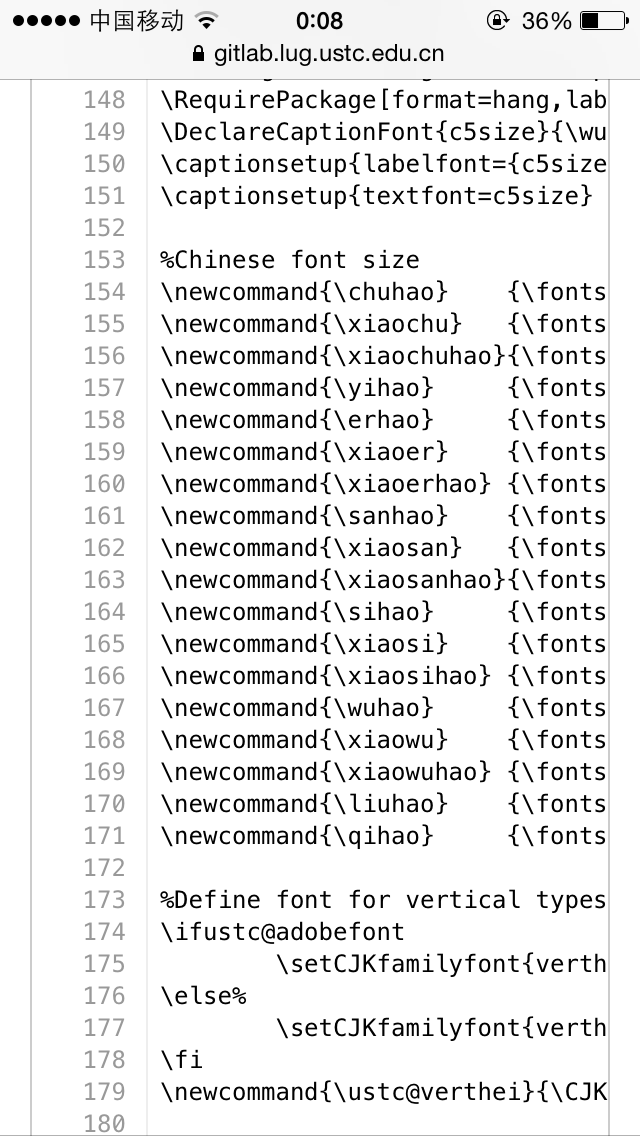
\includegraphics[width=0.6\linewidth]{figure/IMG_1832}
\caption{\LaTeX 字号错误使用范例}
\label{fig:IMG_1832}
\end{figure}
\end{verbatim}
其中第一行的\verb|[thbp!]|是用来规定图片位置的命令\verb|t|表示顶部,\verb|h|表示这里,\verb|b|表示底部,\verb|p|则表示“随便哪儿!”\verb|!|则表示“就是这里!” 在第三行中,规定了图片的尺寸,其方式为限定尺寸宽度为0.6倍行线宽。最后是图片的标题和它的标号,有了它们可以很方便地引用一个图片。

在文档中,虽然我们规定了图片所安放的位置和相对应的顺序,但是图片最终在文档中所呈现的位置和代码中的还是会有差距。这是由于所有的图片实际上都是“浮动” 环境,在设置了图片的大小之后实际上最终的位置还是由文字结束之后可以容纳图片的空间位置所决定的。 如果文档末尾空间不足以填充图片,那么排版系统会自动先将文字填充于这个部分然后再放置我们想要的图片。图片的位置时常让我们感到困惑,如果遇到图片位置的问题可以有几个思路参考:
\begin{itemize}
	\item 更改图片大小,或者宽度。由于大多数情况下我们需要图片等比例缩放,实际上修改宽度和修改图片大小是一样的原理。
	\item 新增一个新的页面,容纳过多的图片。
	\item 合理安排图片的数量,避免做“插图大师”。科研文章都是为了内容服务的,切莫为了字数要求,页数要求而恶意灌图。
\end{itemize}

如图(\ref{fig:IMG_1832})中显示了一个错误的字号显示的方法。
\begin{figure}[h]
\centering
\tdplotsetmaincoords{70}{110}
\begin{tikzpicture}[auto,scale=1,tdplot_main_coords]
\draw[thick,->] (0,0,0) -- (3,0,0) node[anchor=north east]{$x$};
\draw[thick,->] (0,0,0) -- (0,3,0) node[anchor=north west]{$y$};
\draw[thick,->] (0,0,0) -- (0,0,3) node[anchor=south]{$z$};
\draw[thick,->,color=red] (1,0,0)--(1,1.5,0.8) node[midway,name=a]{$ \vec{a} $};
\draw[thick,->,color=red] (1,0,0)--(1,-0.8,1.5) node[midway,name=b]{$ \vec{b} $};
\end{tikzpicture}
\caption{三维向量旋转示意}
\label{fig:3Drot}
\end{figure}

而图(\ref{fig:3Drot})则是用TikZ语言做的图片,比较清晰明了。
\subsubsection{在文档中加入表格}
三线表的使用,见如下代码
\begin{verbatim}
\begin{table}[thbp]
\caption{状态估计算法比较}
\begin{center}
\begin{tabular}{cccc}
\hline  & 卡尔曼滤波 & 神经网络滤波 & 被动无源滤波 \\ 
\hline 模型类型 & 线性 & 线性 & 非线性  \\ 
 参数调校 & 大量 & 几乎没有 & 合理 \\ 
 稳定性 & 满足全局稳定性 & 依赖于模型 & 满足子系统稳定性 \\ 
 算法开销 & 低且可以借助硬件实现  & 高且大量依赖软件平台  & 低且可以借助硬件实现  \\ 
 \hline
\end{tabular} 
\end{center}
\label{tb:filter}
\end{table}
\end{verbatim}
\verb|tabular|后的\verb|cccc|表示四个居中的行元素,\verb|llll|则表示四个居左的行元素,\verb|&|分割行元素,\verb|\\|分割列元素,一个\verb|\hline|就是一条线。
\begin{table}[thbp]
\caption{状态估计算法比较}
\begin{center}
\begin{tabular}{cccc}
\hline  & 卡尔曼滤波 & 神经网络滤波 & 被动无源滤波 \\ 
\hline 模型类型 & 线性 & 线性 & 非线性  \\ 
 参数调校 & 大量 & 几乎没有 & 合理 \\ 
 稳定性 & 满足全局稳定性 & 依赖于模型 & 满足子系统稳定性 \\ 
 算法开销 & 低且可以借助硬件实现  & 高且大量依赖软件平台  & 低且可以借助硬件实现  \\ 
 \hline
\end{tabular} 
\end{center}
\label{tb:filter}
\end{table}

如果遇到表格比较复杂的情况,也不必抓耳挠腮,可以使用诸如\href{http://www.tablesgenerator.com}{在线表格编辑器}之类的小工具帮助我们完成工作。
\subsection{数学公式}

美观简洁的数学公式是\LaTeX 中的一大特点,按照数学公式的类型可以分为标号公式和不标号公式两者。不标号公式有有行内公式和行间公式的两种类型分别类似于,行内公式$ e^{i\pi}+1=0 $ 和\[ \dfrac{d\vec{G}}{dt}=\dot{G_x}\vec{i}+\dot{G_y}\vec{j}+\dot{G_z}\vec{k}+G_x\dot{\vec{i}}+G_y\dot{\vec{j}}+G_z\dot{\vec{k}} \],
分别使用美元符号和方括号命令来表示。 通常在学术论文中正文里的重要公式需要编号,编号的公式类型主要有\verb|equation|,\verb|align|,\verb|split|,\verb|eqnarray| 等类型,能够实现等式,方程组,跨行公式的显示。具体的使用方式见\ref{example}
\subsubsection{一个简单的例子}\label{example}
船舶运动中所涉及的力和速度都可以理解为矢量,按照矢量旋转的方法可以对于坐标系统进行转化。
\begin{lemma}
\label{2Drot} 
存在一个旋转矩阵使得任何两个模相同的二维向量相互转换
\end{lemma}
\begin{proof}
设定向量$\vec{X}=(a_1,b_1),\vec{Y}=(a_2,b_2)$ 存在$ J $使得$ XJ=Y $同时$X=YJ^{-1}$,其中\[  \sqrt{a_1^{2}+b_1^{2}}=\sqrt{a_2^{2}+b_2^{2}}=R \] 
由线性方程组的解可知,当$rank(A,Y)=rank(A)=2$时线性方程组有唯一解,此时矩阵$ J $定义为\textit{旋转矩阵},同时$ J^{-1} $定义为\textit{逆旋转矩阵}.
\end{proof}
\begin{theorem}
\label{rotM}
平面旋转矩阵$ J $只和两向量之间的夹角$ \theta $有关
\end{theorem}

\begin{proof}
$ a_1=Rsin\alpha , b_1=Rcos\alpha~~ .~~ a_2=Rsin\beta ,b_2=Rcos\beta $
展开  $ a_2 $可以得到
\[a_2=Rsin\beta=Rsin(\alpha+\theta)=R(sin\alpha cos\theta +cos\alpha sin \theta)\]  
将$cos\alpha=\dfrac{a_1}{R},sin\alpha=\dfrac{b_1}{R}$代入可以得到\[a_2=a_1 cos\theta-b_1 sin\theta \] 同理\[ b_2=a_1 sin\theta+b_1 cos\theta \] 转换为矩阵形式则为
 \begin{align} \begin{bmatrix}
 a_2\\b_2 
\end{bmatrix}=
\begin{bmatrix}
 cos\theta&-sin\theta\\sin\theta& cos\theta
\end{bmatrix}  
\begin{bmatrix}
 a_1\\b_1 
\end{bmatrix}\end{align}
 最终可以得到
 \begin{align}
 \label{Jc}
  {J}_c=\begin{bmatrix} cos\theta&-sin\theta\\sin\theta& cos\theta
\end{bmatrix} 
\end{align}
 逆时针旋转时

\begin{align}
\label{Jcc}
{J}_{cc} =\begin{bmatrix} cos\theta&sin\theta\\-sin\theta& cos\theta
\end{bmatrix}
\end{align}
\end{proof}
\begin{theorem}
任何两个模相同的三维向量,可以通过旋转矩阵相互转化
\end{theorem}
\begin{figure}[h]
\centering
\tdplotsetmaincoords{70}{110}
\begin{tikzpicture}[auto,scale=1,tdplot_main_coords]
\draw[thick,->] (0,0,0) -- (3,0,0) node[anchor=north east]{$x$};
\draw[thick,->] (0,0,0) -- (0,3,0) node[anchor=north west]{$y$};
\draw[thick,->] (0,0,0) -- (0,0,3) node[anchor=south]{$z$};
\draw[thick,->,color=red] (1,0,0)--(1,1.5,0.8) node[midway,name=a]{$ \vec{a} $};
\draw[thick,->,color=red] (1,0,0)--(1,-0.8,1.5) node[midway,name=b]{$ \vec{b} $};
\end{tikzpicture}
\caption{三维向量旋转示意}
\label{fig:3Drot}
\end{figure}

\subsection{呈列代码}
采用listing宏包可以列代码,在控制文件导演区可以更改listing的设置
来符合MATLAB,Python,C++等不同语言的需求。
\begin{python}
#
import java.util.*;  
public class test {  
    public static void main (String[]args){   
        int day=0;  
        int month=0;  
        int year=0;  
        int sum=0;  
        int leap;     
        System.out.print("请输入年,月,日\n");     
        Scanner input = new Scanner(System.in);  
        year=input.nextInt();  
        month=input.nextInt();  
        day=input.nextInt();  
        switch(month) /*先计算某月以前月份的总天数*/    
        {     
        case 1:  
            sum=0;break;     
        case 2:  
            sum=31;break;     
        case 3:  
            sum=59;break;     
        case 4:  
            sum=90;break;     
        case 5:  
            sum=120;break;     
        case 6:  
            sum=151;break;     
        case 7:  
            sum=181;break;     
        case 8:  
            sum=212;break;     
        case 9:  
            sum=243;break;     
        case 10:  
            sum=273;break;     
        case 11:  
            sum=304;break;     
        case 12:  
            sum=334;break;     
        default:  
            System.out.println("data error");break;  
        }     
        sum=sum+day; /*再加上某天的天数*/    
        if(year%400==0||(year%4==0&&year%100!=0))/*判断是不是闰年*/    
            leap=1;     
        else    
            leap=0;     
        if(leap==1 && month>2)/*如果是闰年且月份大于2,总天数应该加一天*/    
            sum++;     
        System.out.println("It is the the day:"+sum);  
        }  
} 
\end{python}